\documentclass[12pt, onecolumn]{article}

% 引入相关的包
\usepackage{amsmath, listings, fontspec, geometry, graphicx, ctex, color, subfigure, amsfonts, amssymb}
\usepackage{multirow}
\usepackage[table,xcdraw]{xcolor}
\usepackage[ruled]{algorithm2e}
\usepackage[hidelinks]{hyperref}
\usepackage{makecell}

		\usepackage{graphicx}
		\usepackage[most]{tcolorbox}
\hypersetup{
	colorlinks=true,
	linkcolor=red,
	citecolor=red,
}
\usepackage{booktabs}
\usepackage{multirow}
\usepackage{picins}

% 设定页面的尺寸和比例
\geometry{left = 1.5cm, right = 1.5cm, top = 1.5cm, bottom = 1.5cm}

% 设定两栏之间的间距
\setlength\columnsep{1cm}

% 设定字体,为代码的插入作准备
\newfontfamily\ubuntu{Ubuntu Mono}
\newfontfamily\consolas{Consolas}

% 头部信息
\title{\normf{编程:观测值逐次更新的扩展卡尔曼滤波器}}
\author{\normf 姓名:陈烁龙\;\;\;学号:2023202140019\;\;\;学院:测绘学院}
\date{\normf{\today}}

% 代码块的风格设定
\lstset{
	language=C++,
	basicstyle=\footnotesize\ubuntu,
	keywordstyle=\textbf,
	stringstyle=\itshape,
	commentstyle=\itshape,
	numberstyle=\scriptsize\ubuntu,
	showstringspaces=false,
	numbers=left,
	numbersep=8pt,
	tabsize=2,
	frame=single,
	framerule=1pt,
	columns=fullflexible,
	breaklines,
	frame=shadowbox, 
	backgroundcolor=\color[rgb]{0.97,0.97,0.97}
}

% 字体族的定义
% \fangsong \songti \heiti \kaishu
\newcommand\normf{\fangsong}
\newcommand\boldf{\heiti}
\newcommand\keywords[1]{\boldf{关键词:} \normf #1}

\newcommand\liehat[1]{\left[ #1 \right]_\times}
\newcommand\lievee[1]{\left[ #1 \right]^\vee}
\newcommand\liehatvee[1]{\left[ #1 \right]^\vee_\times}

\newcommand\mlcomment[1]{\iffalse #1 \fi}
%\newcommand\mlcomment[1]{ #1 }

\newcounter{problemname}
\newenvironment{problem}{\stepcounter{problemname}\par\noindent\normf\textbf{\textcolor[rgb]{1,0,0}{题目\arabic{problemname}.} }}{\leavevmode\\\par}
\newenvironment{solution}{\par\noindent\normf\textbf{解答: }}{\leavevmode\\\par}
\newenvironment{note}{\par\noindent\normf\textbf{题目\arabic{problemname}的注记: }}{\leavevmode\\\par}


\begin{document}
	\begin{titlepage}
	    \centering
	    
\includegraphics[width=0.4\textwidth]{whu_red.png}\par\vspace{1cm}
	    \vspace{4cm}
	    {\huge\bfseries River \par}
	    \vspace{3cm}
	    {\Large\kaishu 
	    \begin{center}\begin{tabular}{l}
	    姓名:陈烁龙\\
	    学号:\bfseries 2023202140019\\
	    学院:测绘学院
	    \end{tabular}\end{center}
	     \par}
	    
	
	    \vfill
	
	% Bottom of the page
	    {\large\kaishu\bfseries \today\par}
	\end{titlepage}
		% 换页
 		\thispagestyle{empty}
		\clearpage
		
		% 插入目录、图、表并换页
		\pagenumbering{roman}
		\tableofcontents
		\newpage
		\listoffigures
		\newpage
		\listoftables
		% 罗马字母形式的页码
		
		\clearpage
		% 从该页开始计数
		\setcounter{page}{1}
		% 阿拉伯数字形式的页码
		\pagenumbering{arabic}
		
	\section{\normf{IMU因子}}
	\normf\bfseries
	对于IMU,其理想输出和位姿轨迹之间的关系为:
	\begin{equation}
	\label{equ:imu_bspline}
	\begin{cases}
	\begin{aligned}
	{^{b}\boldsymbol{a}(t)}&={^{b_0}_{b}\boldsymbol{R}^\top(t)}\cdot({^{b_0}\ddot{\boldsymbol{p}}_I(t)}-{^{b_0}\boldsymbol{g}})\\
	{^{b}\boldsymbol{\omega}(t)}&={^{b_0}_{b}\boldsymbol{R}^\top(t)}\cdot{^{b_0}_{b}\dot{\boldsymbol{R}}(t)}
	\end{aligned}
	\end{cases}
	\end{equation}
	现考虑IMU零偏,则其输出为:
	\begin{equation}
	\begin{cases}
	\begin{aligned}
		{^{b}}\hat{\boldsymbol{a}}(\tau)&
		={^{b}}\boldsymbol{a}(\tau)+\boldsymbol{b}_a(\tau)+\boldsymbol{n}_a(\tau)
		\\
		{^{b}}\hat{\boldsymbol{\omega}}(\tau)&
		={^{b}}\boldsymbol{\omega}(\tau)+\boldsymbol{b}_g(\tau)+\boldsymbol{n}_g(\tau)
		\end{aligned}
	\end{cases}
	\end{equation}
	其中$\tau$时刻的零偏$\boldsymbol{b}_\omega(\tau)$和$\boldsymbol{b}_a(\tau)$可以通过相应的零偏样条计算得到。通过构建对应的因子,可以优化“旋转样条”、“速度样条”、“加速度计零偏样条”、“陀螺仪零偏样条”、“首帧下的重力向量”。
	
	\section{\normf{Radar因子}}
	
		\subsection{\normf{Radar Static Measurement (V1)}}
		The continuous-time trajectory is the one of other sensor (e.g., IMU), we have:
		\begin{equation}
		{^{b_0}\boldsymbol{p}_t}={^{b_0}_{b}\boldsymbol{R}(\tau)}\cdot{^{b}\boldsymbol{p}_t(\tau)}+{^{b_0}\boldsymbol{p}_{b}(\tau)}
		\end{equation}
		with
		\begin{equation}
		{^{b}\boldsymbol{p}_t(\tau)}={^{b}_{r}\boldsymbol{R}}\cdot{^{r}\boldsymbol{p}_t(\tau)}+{^{b}\boldsymbol{p}_{r}}
		\end{equation}
		then
		\begin{equation}
		{^{b_0}\boldsymbol{p}_t}={^{b_0}_{b}\boldsymbol{R}(\tau)}\cdot{^{b}_{r}\boldsymbol{R}}\cdot{^{r}\boldsymbol{p}_t(\tau)}
		+{^{b_0}_{b}\boldsymbol{R}(\tau)}\cdot{^{b}\boldsymbol{p}_{r}}
		+{^{b_0}\boldsymbol{p}_{b}(\tau)}
		\end{equation}
		differentiate
		\begin{equation}
		{^{b_0}\dot{\boldsymbol{p}}_t}=\boldsymbol{0}_{3\times 1}=
		-\liehat{{^{b_0}_{b}\boldsymbol{R}(\tau)}\cdot{^{b}_{r}\boldsymbol{R}}\cdot{^{r}\boldsymbol{p}_t(\tau)}}\cdot{^{b_0}_{b}\dot{\boldsymbol{R}}(\tau)}
		+{^{b_0}_{b}\boldsymbol{R}(\tau)}\cdot{^{b}_{r}\boldsymbol{R}}\cdot{^{r}\dot{\boldsymbol{p}}_t(\tau)}
		-\liehat{{^{b_0}_{b}\boldsymbol{R}(\tau)}\cdot{^{b}\boldsymbol{p}_{r}}}\cdot{^{b_0}_{b}\dot{\boldsymbol{R}}(\tau)}
		+{^{b_0}\dot{\boldsymbol{p}}_{b}(\tau)}
		\end{equation}
		\begin{equation}
		\boldsymbol{0}_{3\times 1}=
		-\liehat{{^{b}_{r}\boldsymbol{R}}\cdot{^{r}\boldsymbol{p}_t(\tau)}}\cdot{^{b_0}_{b}\boldsymbol{R}^\top(\tau)}\cdot{^{b_0}_{b}\dot{\boldsymbol{R}}(\tau)}
		+{^{b}_{r}\boldsymbol{R}}\cdot{^{r}\dot{\boldsymbol{p}}_t(\tau)}
		-\liehat{{^{b}\boldsymbol{p}_{r}}}\cdot{^{b_0}_{b}\boldsymbol{R}^\top(\tau)}\cdot{^{b_0}_{b}\dot{\boldsymbol{R}}(\tau)}
		+{^{b_0}_{b}\boldsymbol{R}^\top(\tau)}\cdot{^{b_0}\dot{\boldsymbol{p}}_{b}(\tau)}
		\end{equation}
		\begin{equation}
		\boldsymbol{0}_{3\times 1}=
		-\liehat{{^{r}\boldsymbol{p}_t(\tau)}}\cdot{^{b}_{r}\boldsymbol{R}^\top}\cdot{^{b_0}_{b}\boldsymbol{R}^\top(\tau)}\cdot{^{b_0}_{b}\dot{\boldsymbol{R}}(\tau)}
		+{^{r}\dot{\boldsymbol{p}}_t(\tau)}
		-{^{b}_{r}\boldsymbol{R}^\top}\cdot\liehat{{^{b}\boldsymbol{p}_{r}}}\cdot{^{b_0}_{b}\boldsymbol{R}^\top(\tau)}\cdot{^{b_0}_{b}\dot{\boldsymbol{R}}(\tau)}
		+{^{b}_{r}\boldsymbol{R}^\top}\cdot{^{b_0}_{b}\boldsymbol{R}^\top(\tau)}\cdot{^{b_0}\dot{\boldsymbol{p}}_{b}(\tau)}
		\end{equation}
		thus, the velocity of target $\{t\}$ with respect to the radar $\{r\}$ parameterized in $\{r\}$ could be expressed as:
		\begin{equation}
		\label{equ:static_target_vel}
		{^{r}\dot{\boldsymbol{p}}_t(\tau)}=
		\liehat{{^{r}\boldsymbol{p}_t(\tau)}}\cdot{^{b}_{r}\boldsymbol{R}^\top}\cdot{^{b_0}_{b}\boldsymbol{R}^\top(\tau)}\cdot{^{b_0}_{b}\dot{\boldsymbol{R}}(\tau)}
		+{^{b}_{r}\boldsymbol{R}^\top}\cdot\liehat{{^{b}\boldsymbol{p}_{r}}}\cdot{^{b_0}_{b}\boldsymbol{R}^\top(\tau)}\cdot{^{b_0}_{b}\dot{\boldsymbol{R}}(\tau)}
		-{^{b}_{r}\boldsymbol{R}^\top}\cdot{^{b_0}_{b}\boldsymbol{R}^\top(\tau)}\cdot{^{b_0}\dot{\boldsymbol{p}}_{b}(\tau)}
		\end{equation}
		
		\subsection{\normf{Radar Static Measurement (V2)}}
		Considering the extrinsics between the radar and the IMU, we have:
		\begin{equation}
		{^{b_0}{\boldsymbol{p}}_r(\tau)}={^{b_0}_{b}\boldsymbol{R}(\tau)}\cdot{^{b}{\boldsymbol{p}}_r}+{^{b_0}{\boldsymbol{p}}_b(\tau)}
		\end{equation}
		\begin{equation}
		\label{equ:radar_imu_extri}
		{^{b_0}\dot{\boldsymbol{p}}_r(\tau)}=-\liehat{{^{b_0}_{b}\boldsymbol{R}(\tau)}\cdot{^{b}{\boldsymbol{p}}_r}}\cdot{^{b_0}_{b}\dot{\boldsymbol{R}}(\tau)}
		+{^{b_0}\dot{\boldsymbol{p}}_b(\tau)}
		\end{equation}
		thus, the velocity of radar $\{r\}$ with respect to the frame $\{b_0\}$ parameterized in $\{r\}$ could be expressed as:
		\begin{equation}
		\label{equ:radar_vel}
		{^{b}_{r}\boldsymbol{R}^\top}\cdot{^{b_0}_{b}\boldsymbol{R}^\top(\tau)}\cdot{^{b_0}\dot{\boldsymbol{p}}_r(\tau)}=
		{^{b}_{r}\boldsymbol{R}^\top}\cdot{^{b_0}_{b}\boldsymbol{R}^\top(\tau)}\cdot
		\left(
		-\liehat{{^{b_0}_{b}\boldsymbol{R}(\tau)}\cdot{^{b}{\boldsymbol{p}}_r}}\cdot{^{b_0}_{b}\dot{\boldsymbol{R}}(\tau)}
		+{^{b_0}\dot{\boldsymbol{p}}_b(\tau)}
		\right) 
		\end{equation}
		actually, by introducing ${^{r}\boldsymbol{p}_t^\top(\tau)}$ in (\ref{equ:static_target_vel}) and considering (\ref{equ:radar_vel}), we have:
		\begin{equation}
		\begin{aligned}
		{^{r}\boldsymbol{p}_t^\top(\tau)}\cdot{^{r}\dot{\boldsymbol{p}}_t(\tau)}
		&={^{r}\boldsymbol{p}_t^\top(\tau)}\cdot\left( {^{b}_{r}\boldsymbol{R}^\top}\cdot\liehat{{^{b}\boldsymbol{p}_{r}}}\cdot{^{b_0}_{b}\boldsymbol{R}^\top(\tau)}\cdot{^{b_0}_{b}\dot{\boldsymbol{R}}(\tau)}			-{^{b}_{r}\boldsymbol{R}^\top}\cdot{^{b_0}_{b}\boldsymbol{R}^\top(\tau)}\cdot{^{b_0}\dot{\boldsymbol{p}}_{b}(\tau)}\right) 
		\\
		&={^{r}\boldsymbol{p}_t^\top(\tau)}\cdot\left(
		-{^{b}_{r}\boldsymbol{R}^\top}\cdot{^{b_0}_{b}\boldsymbol{R}^\top(\tau)}\cdot{^{b_0}\dot{\boldsymbol{p}}_r(\tau)}
		\right) 
		\\&=-{^{r}\boldsymbol{p}_t^\top(\tau)}\cdot{^{b}_{r}\boldsymbol{R}^\top}\cdot{^{b_0}_{b}\boldsymbol{R}^\top(\tau)}\cdot{^{b_0}\dot{\boldsymbol{p}}_r(\tau)}
		\end{aligned}
		\end{equation}
		thus, we have:
		\begin{equation}
		{^{r}\boldsymbol{p}_t^\top(\tau)}\cdot{^{b}_{r}\boldsymbol{R}^\top}\cdot{^{b_0}_{b}\boldsymbol{R}^\top(\tau)}\cdot{^{b_0}\dot{\boldsymbol{p}}_r(\tau)}=
		-{^{r}\boldsymbol{p}_t^\top(\tau)}\cdot{^{r}\dot{\boldsymbol{p}}_t(\tau)}
		\end{equation}
		\subsection{\normf{因子构建}}
		对于radar量测有:
			\begin{equation}
			\label{equ:radar_model}
			\small
			v=
			\frac{{^{r}\boldsymbol{p}_t^\top}\cdot{^{r}\dot{\boldsymbol{p}}_t}}{d}
			\quad\mathrm{s.t.}\;
			{^{r}\boldsymbol{p}_t}=d\cdot\begin{pmatrix}
			\cos\theta\cos\phi
			\\
			\sin\theta\cos\phi
			\\
			\sin\phi
			\end{pmatrix}
			\end{equation}
		当target是静态的时候,有:
		\begin{equation}
		v\cdot d=-{^{r}\boldsymbol{p}_t^\top(\tau)}\cdot{^{b}_{r}\boldsymbol{R}^\top}\cdot{^{b_0}_{b}\boldsymbol{R}^\top(\tau)}\cdot{^{b_0}\dot{\boldsymbol{p}}_r(\tau)}
		\end{equation}
		通过上式即可构建radar因子。
		
		\section{\normf{初始化}}
		使用速度层面的预积分进行初始化。首先进行旋转样条的拟合以及每一帧radar数据(包含多个target量测)的速度计算。radar帧速度计算通过最小二乘,计算得到${^{b_0}\dot{\boldsymbol{p}}_r(\tau)}$:
		\begin{equation}
		v\cdot d=-
		{^{r}\boldsymbol{p}_t^\top(\tau)}\cdot{^{b}_{r}\boldsymbol{R}^\top}\cdot{^{b_0}_{b}\boldsymbol{R}^\top}(\tau)\cdot{^{b_0}\dot{\boldsymbol{p}}_r(\tau)}
		\end{equation}
		
		对于IMU量测, 基于连续时间的预积分(速度层面),有:
		\begin{equation}
		{^{b}\boldsymbol{a}(t)}={^{b_0}_{b}\boldsymbol{R}^\top(t)}\cdot\left( {^{b_0}\ddot{\boldsymbol{p}}_b(t)}-{^{b_0}\boldsymbol{g}}\right)
		\quad\to\quad
		{^{b_0}_{b}\boldsymbol{R}(t)}\cdot{^{b}\boldsymbol{a}(t)}= {^{b_0}\ddot{\boldsymbol{p}}_b(t)}-{^{b_0}\boldsymbol{g}}
		\end{equation}
		在$\tau\in[t_k,t_{k+1}]$时间段内,有:
		\begin{equation}
		\int_{t_k}^{t_{k+1}}{^{b_0}_{b}\boldsymbol{R}(\tau)}\cdot{^{b}\boldsymbol{a}(\tau)}\cdot d\tau=
		{^{b_0}\dot{\boldsymbol{p}}_b(t_{k+1})}-{^{b_0}\dot{\boldsymbol{p}}_b(t_k)}
		-{^{b_0}\boldsymbol{g}}\cdot (t_{k+1}-t_k)
		\end{equation}
		其中的${^{b_0}\dot{\boldsymbol{p}}_b(t_{k+1})}$和${^{b_0}\dot{\boldsymbol{p}}_b(t_k)}$可以通过(\ref{equ:radar_imu_extri})得到,也即:
		\begin{equation}
		{^{b_0}\dot{\boldsymbol{p}}_b(\tau)}=
		{^{b_0}\dot{\boldsymbol{p}}_r(\tau)}
		+\liehat{{^{b_0}_{b}\boldsymbol{R}(\tau)}\cdot{^{b}{\boldsymbol{p}}_r}}\cdot{^{b_0}_{b}\dot{\boldsymbol{R}}(\tau)}
		\end{equation}
		至此,重力向量即可初始化完成。而后使用IMU因子、radar因子对系统内的所有变量进行refinement。完成后将$\{b_0\}$的负z轴对齐到重力向量方向,将其作为世界参考系$\{w\}$。
		
	\section{\normf{因子加权}}
	IMU量测建模为:
	\begin{equation}
	\begin{cases}
	\begin{aligned}
		{^{b}}\hat{\boldsymbol{a}}(\tau)&
		={^{b}}\boldsymbol{a}(\tau)+\boldsymbol{b}_a(\tau)+\boldsymbol{n}_a(\tau)
		\\
		{^{b}}\hat{\boldsymbol{\omega}}(\tau)&
		={^{b}}\boldsymbol{\omega}(\tau)+\boldsymbol{b}_g(\tau)+\boldsymbol{n}_g(\tau)
		\end{aligned}
	\end{cases}
	\end{equation}
	其中$\boldsymbol{e}_a(\tau)$和$\boldsymbol{e}_g(\tau)$为高斯白噪声:
	\begin{equation}
	\boldsymbol{n}_a(\tau)=\sigma_a\cdot\frac{1}{\sqrt{\Delta \tau}}\cdot\boldsymbol{e}(\tau)
	\qquad
	\boldsymbol{n}_g(\tau)=\sigma_g\cdot\frac{1}{\sqrt{\Delta \tau}}\cdot\boldsymbol{e}(\tau)
	\qquad
	\boldsymbol{e}(\tau)\sim\mathcal{N}(\boldsymbol{0}_{3\times 1},\boldsymbol{I}_3)
	\end{equation}
	且$\sigma_a$的单位为$\left( \begin{aligned}
	\frac{m}{s^2}\times\frac{1}{\sqrt{hz}}
	\end{aligned}\right) $,$\sigma_g$的单位为$\left( \begin{aligned}
		\frac{rad}{s}\times\frac{1}{\sqrt{hz}}
		\end{aligned}\right) $。
	而$\boldsymbol{b}_a(\tau)$和$\boldsymbol{b}_g(\tau)$为零偏,建模为随机游走:
	\begin{equation}
	\dot{\boldsymbol{b}}_a(\tau)=\sigma_{b_a}\cdot\boldsymbol{I}_3\cdot\boldsymbol{e}(\tau)
	\qquad
	\dot{\boldsymbol{b}}_g(\tau)=\sigma_{b_g}\cdot\boldsymbol{I}_3\cdot\boldsymbol{e}(\tau)
	\end{equation}
	且$\sigma_{b_a}$的单位为$\left( \begin{aligned}
		\frac{m}{s^3}\times\frac{1}{\sqrt{hz}}
		\end{aligned}\right) $,$\sigma_{b_g}$的单位为$\left( \begin{aligned}
			\frac{rad}{s^2}\times\frac{1}{\sqrt{hz}}
			\end{aligned}\right) $,对其进行离散化后,有:
	\begin{equation}
	{\boldsymbol{b}}_a(\tau_{k+1})={\boldsymbol{b}}_a(\tau_{k})+\sigma_{b_a}\cdot\sqrt{\Delta \tau}\cdot\boldsymbol{I}_3\cdot\boldsymbol{e}(\tau)
	\end{equation}
	注意,有$\begin{aligned}
	\frac{1}{hz}=\Delta \tau
	\end{aligned}$。
	
	综上,对零偏连续时间状态方程进行离散化,得到:
	\begin{equation}
	\begin{pmatrix}
	{\boldsymbol{b}}_a(\tau_{k+1})\\{\boldsymbol{b}}_g(\tau_{k+1})
	\end{pmatrix}=\begin{pmatrix}
	\boldsymbol{I}_3&\boldsymbol{0}_{3\times 3}\\
	\boldsymbol{0}_{3\times 3}&\boldsymbol{I}_3
	\end{pmatrix}\begin{pmatrix}
	{\boldsymbol{b}}_a(\tau_{k})\\{\boldsymbol{b}}_g(\tau_{k})
	\end{pmatrix}+\sqrt{\Delta \tau}\cdot\begin{pmatrix}
	\sigma_{b_a}\cdot\boldsymbol{I}_3&\boldsymbol{0}_{3\times 3}\\
	\boldsymbol{0}_{3\times 3}&\sigma_{b_a}\cdot\boldsymbol{I}_3
	\end{pmatrix}\begin{pmatrix}
	\boldsymbol{e}(\tau_k)\\\boldsymbol{e}(\tau_k)
	\end{pmatrix}
	\end{equation}
	于是,有:
	\begin{equation}
	\boldsymbol{D}_{\boldsymbol{b}}(\tau_{k+1})=\boldsymbol{D}_{\boldsymbol{b}}(\tau_{k})+\Delta\tau\cdot\begin{pmatrix}
	\sigma_{b_a}^2\cdot\boldsymbol{I}_3&\boldsymbol{0}_{3\times 3}\\
	\boldsymbol{0}_{3\times 3}&\sigma_{b_g}^2\cdot\boldsymbol{I}_3
	\end{pmatrix}
	\end{equation}
	使用的IMU为XSens MTI-G-710,加速度计相关参数为:
	\begin{equation}
	\begin{cases}
	\begin{aligned}
	\sigma_a&=60\left( \frac{\mu g}{\sqrt{hz}}\right) =60\times 10^{-6}\times 9.8\left( \frac{m}{s^2}\times\frac{1}{\sqrt{hz}}\right) =5.880\times 10^{-4}\left( \frac{m}{s^2}\times\frac{1}{\sqrt{hz}}\right) 
	\\
	\sigma_{b_a}&=\cdots
	\end{aligned}
	\end{cases}
	\end{equation}
	陀螺仪相关参数为:
	\begin{equation}
	\begin{cases}
	\begin{aligned}
	\sigma_g&=0.01\left( \frac{deg}{s}\times\frac{1}{\sqrt{hz}}\right) =\frac{0.01\times \pi}{180}\left( \frac{rad}{s}\times\frac{1}{\sqrt{hz}}\right) 
	\approx 1.745\times 10^{-4}\left( \frac{rad}{s}\times\frac{1}{\sqrt{hz}}\right)
	\\
	\sigma_{b_g}&=\cdots
	\end{aligned}
	\end{cases}
	\end{equation}
	
	\section{\normf 基于卡尔曼滤波器的样条先验}
	\subsection{\normf 零偏先验}
	以加速度计零偏为例,$\tau$时刻的零偏为:$\boldsymbol{b}_a(\tau)$。
	则基于速度随机游走模型,容易得到离散化后的状态方程为:
	\begin{equation}
	\boldsymbol{b}_a(\tau_{k+1},\tau_k)=
	\left( \boldsymbol{I}_3\right) \cdot\boldsymbol{b}_a(\tau_{k})
	+\left( \sigma_{b_a}\cdot\sqrt{\Delta \tau}\cdot\boldsymbol{I}_3\right) \cdot\boldsymbol{e}(\tau_k)
	\end{equation}
	其中$\boldsymbol{b}_a(\tau_{k+1},\tau_k)$为第$k+1$时刻的预测状态,$\boldsymbol{b}_a(\tau_{k})$为第$k$个时刻的状态,$\Delta \tau$为时间间隔。方差传播为:
	\begin{equation}
	\boldsymbol{D}_{b_a}(\tau_{k+1},\tau_k)=\boldsymbol{D}_{b_a}(\tau_{k})+\Delta\tau\cdot\sigma_{b_a}^2\cdot\boldsymbol{I}_3
	\end{equation}
	基于得到的第$k+1$个时刻的状态预测和方差信息,在增量优化的时候进行先验信息的约束。优化完成后,得到第$k+1$时刻状态的虚拟量测值$\hat{\boldsymbol{b}}_a(\tau_{k+1})$及其观测方差$\hat{\boldsymbol{D}}(\tau_{k+1})$。而后进行更新操作:
	\begin{equation}
	\begin{aligned}
	\boldsymbol{b}_a(\tau_{k+1})&=\boldsymbol{b}_a(\tau_{k+1},\tau_k)+\boldsymbol{K}(\tau_{k+1})\left(
		\hat{\boldsymbol{b}}_a(\tau_{k+1})-\boldsymbol{b}_a(\tau_{k+1},\tau_k)
		\right) 
		\\
		\boldsymbol{D}_{b_a}(\tau_{k+1})&=\left( \boldsymbol{I}_3-\boldsymbol{K}(\tau_{k+1})\right) \boldsymbol{D}_{b_a}(\tau_{k+1},\tau_k)\left( \boldsymbol{I}_3-\boldsymbol{K}(\tau_{k+1})\right)^\top
		+\boldsymbol{K}(\tau_{k+1})\hat{\boldsymbol{D}}(\tau_{k+1})\boldsymbol{K}^\top(\tau_{k+1})
	\end{aligned}
	\end{equation}
	其中:
	\begin{equation}
	\boldsymbol{K}(\tau_{k+1})=\boldsymbol{D}_{b_a}(\tau_{k+1},\tau_k)\left(\boldsymbol{D}_{b_a}(\tau_{k+1},\tau_k)+\hat{\boldsymbol{D}}(\tau_{k+1}) \right)^{-1}
	\end{equation}
	\subsection{\normf 速度先验}
	
	
	
	
	
	
	\section{\normf{边缘化}}
	\subsection{\normf{ceres四元数求导相关问题}}
	四元数对李代数求导:
	\begin{equation}
	\boldsymbol{q}=
	\begin{pmatrix}
	q_x&q_y&q_z&q_w
	\end{pmatrix} ^\top=\begin{pmatrix}
	\begin{aligned}
	\frac{\boldsymbol{\theta}}{\theta}\sin\frac{\theta}{2}
	\end{aligned}&
	\begin{aligned}
		\cos\frac{\theta}{2}
		\end{aligned}
	\end{pmatrix}
	\end{equation}
	其中:
	\begin{equation}
	\boldsymbol{\theta}=\begin{pmatrix}
	\theta_x&\theta_y&\theta_z
	\end{pmatrix}
	\qquad
	\theta=\sqrt{\left( \theta_x\right) ^2+\left( \theta_y\right) ^2+\left( \theta_z\right) ^2}
	\end{equation}
	于是对于右扰动模型(VINS-Mono使用的,Sophus使用的),有:
	\begin{equation}
	\boldsymbol{q}=\boldsymbol{q}\circ\delta\boldsymbol{q}=\mathcal{L}(\boldsymbol{q})\cdot\begin{bmatrix}
	\begin{aligned}
	\frac{1}{2}\cdot\delta\boldsymbol{\theta}
	\end{aligned}\\1
	\end{bmatrix}
	\qquad
	\frac{\partial \boldsymbol{q}}{\partial \boldsymbol{\theta}}
	=\frac{1}{2}\cdot\mathcal{L}\left(\boldsymbol{q} \right) \cdot\begin{pmatrix}
	\boldsymbol{I}_3&\boldsymbol{0}_3
	\end{pmatrix}^\top=
	\frac{1}{2}\cdot\left( \begin{array}{ccc}
		q_w&-q_z&q_y\\
		q_z&q_w&-q_x\\
		-q_y&q_x&q_w\\
		\hline
		-q_x&-q_y&-q_z
	\end{array}\right)
	\end{equation}
	其中$\mathcal{L}\left(\boldsymbol{q} \right)$为$\boldsymbol{q}$对应的左乘矩阵:
	\begin{equation}
	\mathcal{L}\left(\boldsymbol{q} \right)=\begin{pmatrix}
	q_w\cdot\boldsymbol{I}_3+\liehat{\boldsymbol{q}_v}&\boldsymbol{q}_v\\
	-\boldsymbol{q}_v^\top&q_w
	\end{pmatrix}=\left( \begin{array}{ccc|c}
	q_w&-q_z&q_y&q_x\\
	q_z&q_w&-q_x&q_y\\
	-q_y&q_x&q_w&q_z\\
	\hline
	-q_x&-q_y&-q_z&q_w
	\end{array}\right) 
	\end{equation}
	同样可以推到得到左扰动模型导数为(Ceres使用的):
	\begin{equation}
	\boldsymbol{q}=\delta\boldsymbol{q}\circ\boldsymbol{q}=\mathcal{R}(\boldsymbol{q})\cdot\begin{bmatrix}
	\begin{aligned}
	\frac{1}{2}\cdot\delta\boldsymbol{\theta}
	\end{aligned}\\1
	\end{bmatrix}
	\qquad
		\frac{\partial \boldsymbol{q}}{\partial \boldsymbol{\theta}}
		=\frac{1}{2}\cdot\mathcal{R}\left(\boldsymbol{q} \right) \cdot\begin{pmatrix}
		\boldsymbol{I}_3&\boldsymbol{0}_3
		\end{pmatrix}^\top=
		\frac{1}{2}\cdot\left( \begin{array}{ccc}
			q_w&q_z&-q_y\\
			-q_z&q_w&q_x\\
			q_y&-q_x&q_w\\
			\hline
			-q_x&-q_y&-q_z
		\end{array}\right)
	\end{equation}


	\subsection{\normf{ceres评估函数}}
	参数块的Global Size指的是其实际大小,比如用四元素表示的旋转有4个参数,三维系下的重力向量有3个参数。参数块的Local Size指的是其自由度,比如用四元素表示的旋转有3个自由度(单位四元数模长为1),三维系下的重力向量有2个自由度(重力向量模长为9.8)。不在流形上进行优化的参数的Global Size和Local Size相同, 比如位移状态向量。
	
	参数快的尺寸直接决定了求解的雅克比矩阵的大小,ceres提供了两者求解雅可比矩阵的方法:
	\begin{lstlisting}[caption=\normf{Problem类的提供的雅克比矩阵求解}]
	bool Problem::Evaluate(const EvaluateOptions& options, double* cost,
	                std::vector<double>* residuals, std::vector<double>* gradient,
	                CRSMatrix* jacobian);
	\end{lstlisting}
	Key points:
	\begin{enumerate}
	\item Evaluate Problem. Any of the output pointers can be nullptr. Which residual
	blocks and parameter blocks are used is controlled by the EvaluateOptions
	struct.
	
	\begin{lstlisting}[caption=EvaluateOptions]
	// Options struct to control Problem::Evaluate.
	  struct EvaluateOptions {
	    // The set of parameter blocks for which evaluation should be
	    // performed. This vector determines the order that parameter blocks occur
	    // in the gradient vector and in the columns of the jacobian matrix. If
	    // parameter_blocks is empty, then it is assumed to be equal to vector
	    // containing ALL the parameter blocks. Generally speaking the parameter
	    // blocks will occur in the order in which they were added to the
	    // problem. But, this may change if the user removes any parameter blocks
	    // from the problem.
	    //
	    // NOTE: This vector should contain the same pointers as the ones used to
	    // add parameter blocks to the Problem. These parameter block should NOT
	    // point to new memory locations. Bad things will happen otherwise.
	    std::vector<double*> parameter_blocks;
	
	    // The set of residual blocks to evaluate. This vector determines the order
	    // in which the residuals occur, and how the rows of the jacobian are
	    // ordered. If residual_blocks is empty, then it is assumed to be equal to
	    // the vector containing ALL the residual blocks. Generally speaking the
	    // residual blocks will occur in the order in which they were added to the
	    // problem. But, this may change if the user removes any residual blocks
	    // from the problem.
	    std::vector<ResidualBlockId> residual_blocks;
	
	    // Even though the residual blocks in the problem may contain loss
	    // functions, setting apply_loss_function to false will turn off the
	    // application of the loss function to the output of the cost function. This
	    // is of use for example if the user wishes to analyse the solution quality
	    // by studying the distribution of residuals before and after the solve.
	    bool apply_loss_function = true;
	
	    int num_threads = 1;
	  };
	\end{lstlisting}
	
	\item The evaluation will use the values stored in the memory locations
	pointed to by the parameter block pointers used at the time of the
	construction of the problem.
	
	\item If no LocalParameterizations or Manifolds are used, then the size
	of the gradient vector (and the number of columns in the jacobian) is the
	sum of the sizes of all the parameter blocks. If a parameter block has a
	LocalParameterization or Manifold, then it contributes “TangentSize”
	entries to the gradient vector (and the number of columns in the jacobian).
	\end{enumerate}
	
	\begin{lstlisting}[caption=\normf{CostFunction类的提供的雅克比矩阵求解}]
  virtual bool CostFunction::Evaluate(double const* const* parameters,
                        double* residuals, double** jacobians) const = 0;
	\end{lstlisting}
	Key points:
	\begin{enumerate}
	\item parameters has the same number of
	elements as parameter-block-sizes.  Parameter blocks are in the
	same order as parameter-block-sizes.
	
	\item A more interesting and common use is to impose constraints on the
	parameters. If the initial values of the parameter blocks satisfy
	the constraints, then returning false whenever the constraints
	are not satisfied will prevent the solver from moving into the
	infeasible region. This is not a very sophisticated mechanism for
	enforcing constraints, but is often good enough.
	\end{enumerate}
	
	二者最主要的区别在于CostFunction类的提供的雅克比矩阵求解只考虑了参数块的Global Size,而Problem类的提供的雅克比矩阵求解考虑参数块Local Size。最主要的原因是Problem类知道参数块的流形优化信息,所以可以提供更进一步的雅克比矩阵。
	\begin{lstlisting}[caption=\normf{流形优化}]
        Problem::SetManifold(gravity, new ceres::SphereManifold<3>());
        Problem::SetManifold(SO3_BiToBc, new ceres::EigenQuaternionManifold());
	\end{lstlisting}
	
	与此类似的,当为某个残差函数(cost function)指定损失函数(loss function)的时候,Problem类知道,但是CostFunction类不知道,所以恢复得到的残差向量中,Problem类得到的包含了损失函数信息,所以如果是由CostFunction类计算得到的残差信息,需要通过损失函数映射残差。具体参考ceres官网(\url{http://www.ceres-solver.org/nnls_modeling.html#lossfunction})。
	
	\subsection{\normf{舒尔补}}
	使用ceres优化,每次迭代优化求解线性方程组:
	\begin{equation}
	\left( \boldsymbol{J}^\top\boldsymbol{J}\right) \cdot\delta\boldsymbol{x}=
	\left( -\boldsymbol{J}^\top\boldsymbol{e}\right) 
	\Rightarrow
	\boldsymbol{H}\cdot\delta\boldsymbol{x}=\boldsymbol{b}
	\end{equation}
	现令$\delta\boldsymbol{x}$由待边缘化的状态$\delta\boldsymbol{x}_m$和不边缘化的状态$\delta\boldsymbol{x}_n$构成,则有:
	\begin{equation}
	\begin{pmatrix}
	\boldsymbol{h}_{mm}&\boldsymbol{h}_{mn}\\
	\boldsymbol{h}_{nm}&\boldsymbol{h}_{nn}
	\end{pmatrix}\cdot\begin{pmatrix}
	\delta\boldsymbol{x}_m\\
	\delta\boldsymbol{x}_n
	\end{pmatrix}=\begin{pmatrix}
	\boldsymbol{b}_{m}\\\boldsymbol{b}_{n}
	\end{pmatrix}
	\end{equation}
	对上式进行等价变换:
	\begin{equation}
	\left( \begin{array}{cc|c}
	\boldsymbol{h}_{mm}&\boldsymbol{h}_{mn}&\boldsymbol{b}_m\\
	\boldsymbol{h}_{nm}&\boldsymbol{h}_{nn}&\boldsymbol{b}_n
	\end{array}\right) 
	\xrightarrow{r_2-\boldsymbol{h}_{nm}\cdot\boldsymbol{h}_{mm}^{-1}\cdot r_1}
	\left( \begin{array}{cc|cc}
	\boldsymbol{h}_{mm}&\boldsymbol{h}_{mn}&\boldsymbol{b}_m\\
	\boldsymbol{0}_{nm}&\boldsymbol{h}_{nn}-\boldsymbol{h}_{nm}\cdot\boldsymbol{h}_{mm}^{-1}\cdot\boldsymbol{h}_{mn}
	&
	\boldsymbol{b}_n-\boldsymbol{h}_{nm}\cdot\boldsymbol{h}_{mm}^{-1}\cdot\boldsymbol{b}_{m}
	\end{array}\right) 
	\end{equation}
	最终得到:
	\begin{equation}
	\left(
	\boldsymbol{h}_{nn}-\boldsymbol{h}_{nm}\cdot\boldsymbol{h}_{mm}^{-1}\cdot\boldsymbol{h}_{mn}\right) \cdot\delta\boldsymbol{x}_n=	\boldsymbol{b}_n-\boldsymbol{h}_{nm}\cdot\boldsymbol{h}_{mm}^{-1}\cdot\boldsymbol{b}_{m}
	\Rightarrow
	\boldsymbol{H}_*\cdot\delta\boldsymbol{x}_n=\boldsymbol{b}_*
	\end{equation}
	注意到,上式中的$\boldsymbol{H}_*$和$\boldsymbol{b}_*$是基于当前状态计算得到的。当$\boldsymbol{x}$变化的时候,二者也会发生变化。
	为此,对$\boldsymbol{b}^*$进行线性化操作:
	\begin{equation}
	\boldsymbol{b}^{(k+1)}=\boldsymbol{b}^{(k)}+\frac{\partial \boldsymbol{b}}{\partial\boldsymbol{x}}\cdot\delta\boldsymbol{x}=
	\boldsymbol{b}^{(k)}+\frac{\partial \boldsymbol{b}}{\partial\boldsymbol{e}}\cdot\frac{\partial \boldsymbol{e}}{\partial\boldsymbol{x}}\cdot\delta\boldsymbol{x}=
	\boldsymbol{b}^{(k)}-\boldsymbol{J}^\top\boldsymbol{J}\cdot\delta\boldsymbol{x}=\boldsymbol{b}^{(k)}-\boldsymbol{H}\cdot\delta\boldsymbol{x}
	\end{equation}
	由此得到:
	\begin{equation}
	\begin{cases}
	\begin{aligned}
	\boldsymbol{b}_m^{(k+1)}&=\boldsymbol{b}_m^{(k)}-\boldsymbol{h}_{mm}\cdot\delta\boldsymbol{x}_m-\boldsymbol{h}_{mn}\cdot\delta\boldsymbol{x}_n
	\\
	\boldsymbol{b}_n^{(k+1)}&=\boldsymbol{b}_n^{(k)}-\boldsymbol{h}_{nm}\cdot\delta\boldsymbol{x}_m-\boldsymbol{h}_{nn}\cdot\delta\boldsymbol{x}_n
	\end{aligned}
	\end{cases}
	\end{equation}
	即有:
	\begin{equation}
	\begin{aligned}
	\boldsymbol{b}^{(k+1)}_*&=\boldsymbol{b}_n^{(k+1)}-\boldsymbol{h}_{nm}\cdot\boldsymbol{h}_{mm}^{-1}\cdot\boldsymbol{b}_{m}^{(k+1)}
	\\
	&=\left( \boldsymbol{b}_n^{(k)}-\boldsymbol{h}_{nm}\cdot\delta\boldsymbol{x}_m-\boldsymbol{h}_{nn}\cdot\delta\boldsymbol{x}_n\right) -\boldsymbol{h}_{nm}\cdot\boldsymbol{h}_{mm}^{-1}\cdot\left(
	\boldsymbol{b}_m^{(k)}-\boldsymbol{h}_{mm}\cdot\delta\boldsymbol{x}_m-\boldsymbol{h}_{mn}\cdot\delta\boldsymbol{x}_n
	\right) 
	\\
	&=\left( \boldsymbol{b}_n^{(k)}-\boldsymbol{h}_{nm}\cdot\boldsymbol{h}_{mm}^{-1}\cdot\boldsymbol{b}_m^{(k)}\right) -\left( \boldsymbol{h}_{nn}-\boldsymbol{h}_{nm}\cdot\boldsymbol{h}_{mm}^{-1}\cdot\boldsymbol{h}_{mn}\right) \cdot\delta\boldsymbol{x}_n
	\\
	&=\boldsymbol{b}_*^{(k)}-\boldsymbol{H}_*\cdot\delta\boldsymbol{x}_n
	\end{aligned}
	\end{equation}
	对上式进一步化简,得到:
	\begin{equation}
	\boldsymbol{b}^{(k+1)}_*=\boldsymbol{b}_*^{(k)}-\boldsymbol{H}_*\cdot\delta\boldsymbol{x}_n=\boldsymbol{J}_*^\top\cdot\left(\left( {\boldsymbol{J}_*^\top}\right) ^{-1}\cdot\boldsymbol{b}_*^{(k)} -\boldsymbol{J}_*\cdot\delta\boldsymbol{x}_n\right) 
	\end{equation}
	所以残差为:
	\begin{equation}
	\boldsymbol{e}_*=-\left( \left( {\boldsymbol{J}_*^\top}\right) ^{-1}\cdot\boldsymbol{b}_*^{(k)} -\boldsymbol{J}_*\cdot\delta\boldsymbol{x}_n\right) =\boldsymbol{J}_*\cdot\delta\boldsymbol{x}_n-\left( {\boldsymbol{J}_*^\top}\right) ^{-1}\cdot\boldsymbol{b}_*^{(k)}
	\end{equation}
	
	\subsection{\normf{测试案例}}
	Consider now a slightly more complicated example – the minimization of Powell’s function. Let $\boldsymbol{x}=\left( x_1,x_2,x_3,x_4\right) ^\top$ and
	\begin{equation}
	\begin{aligned}
	e_1(\boldsymbol{x})&=x_1+10x_2\\
	e_2(\boldsymbol{x})&=\sqrt{5}\left( x_3-x_4\right) \\
	e_3(\boldsymbol{x})&=\left(x_2-2x_3 \right) ^2\\
	e_4(\boldsymbol{x})&=\sqrt{10}\left( x_1-x_4\right) ^2
	\end{aligned}
	\end{equation}
	容易得到:
	\begin{equation}
	\boldsymbol{J}=\begin{pmatrix}
	1&10&0&0\\
	0&0&\sqrt{5}&-\sqrt{5}\\
	0&2\left( x_2-2x_3\right) &-4\left( x_2-2x_3\right) &0\\
	2\sqrt{10}\left(x_1-x_4 \right) &0&0&-2\sqrt{10}\left(x_1-x_4 \right)
	\end{pmatrix}
	\end{equation}
	现在边缘化$x_2$和$x_4$,重排参数向量为$\boldsymbol{x}=\left( x_2,x_4\;\vline\; x_1,x_3\right) ^\top$,则有:
	\begin{equation}
	\boldsymbol{J}=\left( \begin{array}{cc|cc}
	10&0&1&0\\
	0&-\sqrt{5}&0&\sqrt{5}\\
	2\left( x_2-2x_3\right)&0&0&-4\left( x_2-2x_3\right)\\
	0&-2\sqrt{10}\left(x_1-x_4 \right)&2\sqrt{10}\left(x_1-x_4 \right) &0
	\end{array}\right) 
	\end{equation}
	当取$\boldsymbol{x}=\left( x_2,x_4\;\vline\; x_1,x_3\right) ^\top=\left( -1,1\;\vline\; 3,0\right) ^\top$时:
	\begin{equation}
	\boldsymbol{J}=\left( \begin{array}{cc|cc}
	10&0&1&0\\
	0&-\sqrt{5}&0&\sqrt{5}\\
	-2&0&0&4\\
	0&-4\sqrt{10}&4\sqrt{10}&0
	\end{array}\right) 
	\qquad
	\boldsymbol{H}=\boldsymbol{J}^\top\boldsymbol{J}=\left( \begin{array}{cc|cc}
	104&0&10&-8\\
	0&165&-160&-5\\
	\hline
	10&-160&161&0\\
	-8&-5&0&21
	\end{array}\right) 
	\end{equation}
	\begin{equation}
	\boldsymbol{e}=\begin{pmatrix}
	-7&-\sqrt{5}&1&4\sqrt{10}
	\end{pmatrix}^\top
	\qquad
	\boldsymbol{b}=-\boldsymbol{J}^\top\cdot\boldsymbol{e}=\begin{pmatrix}
	72&155&-153&1
	\end{pmatrix}^\top
	\end{equation}
	\begin{equation}
	\boldsymbol{J}_*=\begin{pmatrix}
	-1.90881 &-0.47586\\
	1.11507 &-4.47288\\
	\end{pmatrix}
	\qquad
	\left( {\boldsymbol{J}_*^\top}\right) ^{-1}\cdot\boldsymbol{b}_*=\begin{pmatrix}
	3.36340\\
	-2.86972
	\end{pmatrix}
	\end{equation}
	
	\section{\normf 速度可视化}
	对于世界坐标系$\{w\}$下的某个点${^w\boldsymbol{p}}$,有:
	\begin{equation}
	{^w\boldsymbol{p}}={^w_b\boldsymbol{R}(\tau)}\cdot{^b\boldsymbol{p}}(\tau)+{^w\boldsymbol{p}_b}(\tau)
	\end{equation}
	对时间求导,有(考虑世界系下的点是静止的):
	\begin{equation}
	{^w\dot{\boldsymbol{p}}}=
	-\liehat{{^w_b\boldsymbol{R}(\tau)}\cdot{^b\boldsymbol{p}}(\tau)}\cdot{^w_b\dot{\boldsymbol{R}}(\tau)}
	+{^w_b\boldsymbol{R}(\tau)}\cdot{^b\dot{\boldsymbol{p}}}(\tau)
	+{^w\dot{\boldsymbol{p}}_b}(\tau)=\boldsymbol{0}_{3\times 1}
	\end{equation}
	得到该点相对于$\{b\}$系的线速度在$\{b\}$系下的表示:
	\begin{equation}
	{^b\dot{\boldsymbol{p}}}(\tau)=
	{^w_b\boldsymbol{R}^\top(\tau)}\cdot\left( \liehat{{^w_b\boldsymbol{R}(\tau)}\cdot{^b\boldsymbol{p}}(\tau)}\cdot{^w_b\dot{\boldsymbol{R}}(\tau)}
	-{^w\dot{\boldsymbol{p}}_b}(\tau)\right) 
	\end{equation}
	注:事实上,只需要将速度绘制到$\{w\}$系下就行,OpenGL会通过相机投影转到相机坐标系下。
	
	\section{\normf{样条解析求导}}
	以4阶样条为例,$\mathbb{R}^3$空间下的样条可以表示为:
	\begin{equation}
	\boldsymbol{p}(u)=\begin{pmatrix}
	\boldsymbol{p}_i&\boldsymbol{p}_{i+1}&\boldsymbol{p}_{i+2}&\boldsymbol{p}_{i+3}
	\end{pmatrix}\cdot\boldsymbol{M}^{(k)}\cdot\boldsymbol{u}
	\end{equation}
	其中:
	\begin{equation}
	u=\frac{t-t_0}{\Delta t}-i\qquad\boldsymbol{u}=\begin{pmatrix}
	u^0&u^1&u^2&u^3
	\end{pmatrix}^\top\qquad\boldsymbol{M}^{(k)}=\frac{1}{6}\times\begin{pmatrix}
	 1 &-3 & 3& -1\\
	 4 & 0 &-6&  3\\
	 1 & 3 & 3& -3\\
	 0 & 0 & 0&  1\\
	\end{pmatrix}
	\end{equation}
	$\boldsymbol{M}^{(k)}$称之为blending matrix。由于后面需要用到$\boldsymbol{u}$对时间的导数,所以事先计算其系数Base Coefficients:
	\begin{equation}
	\frac{\partial \boldsymbol{u}}{\partial u}=\begin{pmatrix}
	u^0&u^1&u^2&u^3\\
	0&u^0&2u^1&3u^2\\
	0&0&2u^0&6u^1\\
	0&0&0&6u^0
	\end{pmatrix}\Rightarrow\begin{pmatrix}
	1& 1& 1& 1\\
	0& 1& 2& 3\\
	0& 0& 2& 6\\
	0& 0& 0& 6\\
	\end{pmatrix}
	\end{equation}
	当然,该样条也可以表示为以下的形式:
	\begin{equation}
	\boldsymbol{p}(u)=\begin{pmatrix}
	\boldsymbol{p}_i&\boldsymbol{p}_{i+1}-\boldsymbol{p}_i&\boldsymbol{p}_{i+2}-\boldsymbol{p}_{i+1}&\boldsymbol{p}_{i+3}-\boldsymbol{p}_{i+2}
	\end{pmatrix}\cdot\boldsymbol{\widetilde{M}}^{(k)}\cdot\boldsymbol{u}
	\end{equation}
	此时,$\boldsymbol{\widetilde{M}}^{(k)}$为blending matrix的累加形式,即$\widetilde{m}^{(k)}_{j,n}=\sum_{s=j}^{k-1}m^{(k)}_{s,n}$,有:
	\begin{equation}
	\boldsymbol{\widetilde{M}}^{(k)}=\frac{1}{6}\times\begin{pmatrix}
		 6&  0&  0 & 0\\
		 5 & 3& -3 & 1\\
		 1&  3&  3 &-2\\
		 0 & 0&  0 & 1
		\end{pmatrix}
	\end{equation}
	此时,$\boldsymbol{\widetilde{M}}^{(k)}$的第一行为第一基元向量,本文使用blending matrix。
	
	当计算样条的时间导数时,实际上是对$\boldsymbol{u}$向量求时间导数。以一阶导为例:
	\begin{equation}
	\dot{\boldsymbol{p}}(t)=\frac{\partial \boldsymbol{p}(u)}{\partial t}=
	\begin{pmatrix}
		\boldsymbol{p}_i&\boldsymbol{p}_{i+1}&\boldsymbol{p}_{i+2}&\boldsymbol{p}_{i+3}
		\end{pmatrix}\cdot\boldsymbol{M}^{(k)}\cdot\frac{\partial \boldsymbol{u}}{\partial u}\cdot\frac{\partial u}{\partial t}
	\end{equation}
	其中$\begin{aligned}
	\frac{\partial \boldsymbol{u}}{\partial u}
	\end{aligned}$直接可以基于之前计算得到的Base Coefficients获得,而$\begin{aligned}
	\frac{\partial u}{\partial t}=\frac{1}{\Delta t}
	\end{aligned}$。
	
	
	
	
	
	
	
	
	
	
	
	
	\newpage
	\section{ACKNOWLEDGMENT}
	\begin{tcolorbox}[colback=white,colframe=white!70!black,title={\bfseries Author Information}]
	\par\noindent
		\parbox[t]{\linewidth}{
	 \noindent\parpic{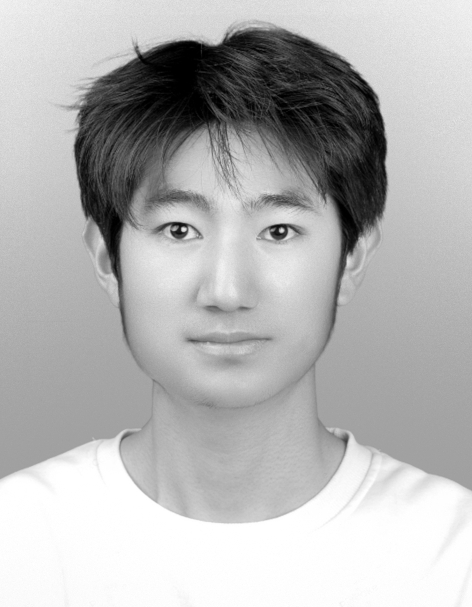
\includegraphics[height=2in,width=1in,clip,keepaspectratio]{ShuolongChen_grey.jpg}}
	 \noindent{\bfseries Shuolong Chen}\emph{
	 received the B.S. degree in geodesy and geomatics engineering from Wuhan University, Wuhan China, in 2023.
	 He is currently a master candidate at the school of Geodesy and Geomatics, Wuhan University. His area of research currently focuses on integrated navigation systems and multi-sensor fusion.
	 Contact him via e-mail: shlchen@whu.edu.cn.
	 }}
	\end{tcolorbox}
		
		
\end{document}

